% ASCE Architecture Diagram — self-contained tikzpicture
% Usage: % ASCE Architecture Diagram — self-contained tikzpicture
% Usage: % ASCE Architecture Diagram — self-contained tikzpicture
% Usage: % ASCE Architecture Diagram — self-contained tikzpicture
% Usage: \input{asce_architecture.tex} inside a figure environment
% Requires: \usepackage{tikz} in the preamble
% Designed for NeurIPS two-column layout (\columnwidth ~ 3.25in)
\usetikzlibrary{arrows.meta, positioning, calc, backgrounds, fit}

% ---------------------------------------------------------------------------
% Colour palette
% ---------------------------------------------------------------------------
\definecolor{ascBlue}{HTML}{4393C3}
\definecolor{ascBlueFill}{HTML}{DAEAF6}
\definecolor{ascRed}{HTML}{C75B39}
\definecolor{ascRedFill}{HTML}{FBEAE4}
\definecolor{ascGreen}{HTML}{388E5E}
\definecolor{ascGreenFill}{HTML}{DFF0E7}
\definecolor{ascYellow}{HTML}{C8A028}
\definecolor{ascYellowFill}{HTML}{FFF3E0}
\definecolor{ascGrey}{HTML}{888888}
\definecolor{ascGreyFill}{HTML}{F0F0F0}

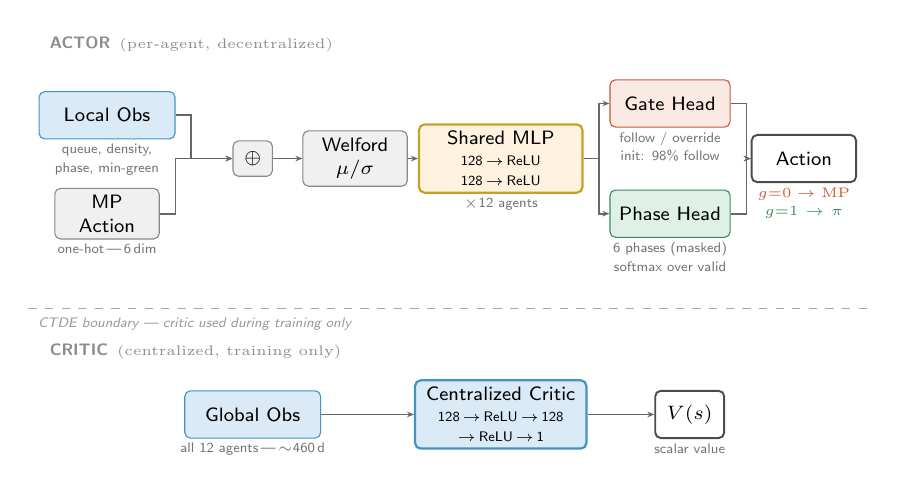
\begin{tikzpicture}[
    x=1cm, y=1cm,
    >={Stealth[length=2.5pt, width=2pt]},
    every node/.style={font=\sffamily},
    % --- node styles ---
    box/.style={
        draw, rounded corners=2pt, minimum height=0.6cm,
        inner sep=2.5pt, align=center,
        font=\sffamily\fontsize{7}{8.4}\selectfont,
    },
    inputbox/.style={box, fill=ascBlueFill, draw=ascBlue, text width=1.55cm},
    greybox/.style={box, fill=ascGreyFill, draw=ascGrey, minimum width=0.7cm},
    mlpbox/.style={box, fill=ascYellowFill, draw=ascYellow, line width=0.8pt,
                   text width=1.9cm, minimum height=0.8cm},
    gatebox/.style={box, fill=ascRedFill, draw=ascRed, text width=1.35cm},
    phasebox/.style={box, fill=ascGreenFill, draw=ascGreen, text width=1.35cm},
    actionbox/.style={box, draw=black!70, line width=0.7pt, text width=1.15cm},
    criticbox/.style={box, fill=ascBlueFill, draw=ascBlue, line width=0.8pt,
                      text width=2.0cm, minimum height=0.8cm},
    % --- annotation styles ---
    sub/.style={font=\sffamily\fontsize{5.5}{6.6}\selectfont,
                text=black!55, align=center, inner sep=0pt},
    arr/.style={->, semithick, color=black!60},
    trk/.style={font=\sffamily\bfseries\fontsize{6.5}{7.8}\selectfont,
                text=black!45},
]

% ===== ACTOR TRACK ==========================================================

\node[trk, anchor=west] at (0.15, 0.9)
    {ACTOR\enspace{\normalfont\fontsize{5.5}{6.6}\selectfont(per-agent, decentralized)}};

% -- Local Obs --
\node[inputbox] (lobs) at (1.0, 0) {Local Obs};
\node[sub, below=1.5pt of lobs.south, anchor=north, text width=2.0cm]
    {queue, density,\\phase, min-green};

% -- MP Action --
\node[greybox, text width=1.15cm] (mpact) at (1.0, -1.25) {MP Action};
\node[sub, below=1.5pt of mpact.south, anchor=north, text width=1.5cm]
    {one-hot\,|\,6\,dim};

% -- Concat --
\node[greybox, minimum width=0.5cm, minimum height=0.45cm,
      font=\sffamily\fontsize{7}{8.4}\selectfont] (cat) at (2.85, -0.55)
    {$\oplus$};

% -- Welford --
\node[greybox, text width=1.15cm] (welf) at (4.15, -0.55)
    {Welford $\mu/\sigma$};

% -- Shared MLP --
\node[mlpbox] (mlp) at (6.0, -0.55)
    {Shared MLP\\[-1pt]
     {\fontsize{5.5}{6.6}\selectfont 128\,$\to$\,ReLU}\\[-1pt]
     {\fontsize{5.5}{6.6}\selectfont 128\,$\to$\,ReLU}};
\node[sub, below=1.5pt of mlp.south, anchor=north]
    {$\times$12 agents};

% -- Gate Head --
\node[gatebox] (gate) at (8.15, 0.15) {Gate Head};
\node[sub, below=1.5pt of gate.south, anchor=north, text width=1.8cm]
    {follow / override\\init: 98\% follow};

% -- Phase Head --
\node[phasebox] (phase) at (8.15, -1.25) {Phase Head};
\node[sub, below=1.5pt of phase.south, anchor=north, text width=1.8cm]
    {6 phases (masked)\\softmax over valid};

% -- Action --
\node[actionbox] (act) at (9.85, -0.55) {Action};
\node[sub, below=1.5pt of act.south, anchor=north, text width=1.6cm]
    {{\color{ascRed}$g{=}0\!\to\!\mathrm{MP}$}\\
     {\color{ascGreen}$g{=}1\!\to\!\pi$}};

% -- Arrows: actor track --
\draw[arr] (lobs.east)  -- ++(0.2,0) |- (cat.west);
\draw[arr] (mpact.east) -- ++(0.2,0) |- (cat.west);
\draw[arr] (cat.east)   -- (welf.west);
\draw[arr] (welf.east)  -- (mlp.west);
\draw[arr] (mlp.east)   -- ++(0.2,0) |- (gate.west);
\draw[arr] (mlp.east)   -- ++(0.2,0) |- (phase.west);
\draw[arr] (gate.east)  -- ++(0.2,0) |- (act.west);
\draw[arr] (phase.east) -- ++(0.2,0) |- (act.west);


% ===== CTDE BOUNDARY ========================================================
\draw[dashed, black!35, line width=0.45pt] (0.0, -2.45) -- (10.7, -2.45);
\node[font=\sffamily\itshape\fontsize{5.5}{6.6}\selectfont, text=black!40,
      anchor=west] at (0.0, -2.65)
    {CTDE boundary --- critic used during training only};


% ===== CRITIC TRACK ==========================================================

\node[trk, anchor=west] at (0.15, -3.0)
    {CRITIC\enspace{\normalfont\fontsize{5.5}{6.6}\selectfont(centralized, training only)}};

% -- Global Obs --
\node[inputbox] (gobs) at (2.85, -3.8) {Global Obs};
\node[sub, below=1.5pt of gobs.south, anchor=north, text width=2.2cm]
    {all 12 agents\,|\,${\sim}$460\,d};

% -- Centralized Critic --
\node[criticbox] (crit) at (6.0, -3.8)
    {Centralized Critic\\[-1pt]
     {\fontsize{5.5}{6.6}\selectfont 128\,$\to$\,ReLU\,$\to$\,128}\\[-1pt]
     {\fontsize{5.5}{6.6}\selectfont $\to$\,ReLU\,$\to$\,1}};

% -- V(s) --
\node[actionbox, text width=0.7cm, minimum width=0.7cm] (vs) at (8.4, -3.8)
    {$V(s)$};
\node[sub, below=1.5pt of vs.south, anchor=north, text width=1.1cm]
    {scalar value};

% -- Arrows: critic track --
\draw[arr] (gobs.east) -- (crit.west);
\draw[arr] (crit.east) -- (vs.west);

\end{tikzpicture}
 inside a figure environment
% Requires: \usepackage{tikz} in the preamble
% Designed for NeurIPS two-column layout (\columnwidth ~ 3.25in)
\usetikzlibrary{arrows.meta, positioning, calc, backgrounds, fit}

% ---------------------------------------------------------------------------
% Colour palette
% ---------------------------------------------------------------------------
\definecolor{ascBlue}{HTML}{4393C3}
\definecolor{ascBlueFill}{HTML}{DAEAF6}
\definecolor{ascRed}{HTML}{C75B39}
\definecolor{ascRedFill}{HTML}{FBEAE4}
\definecolor{ascGreen}{HTML}{388E5E}
\definecolor{ascGreenFill}{HTML}{DFF0E7}
\definecolor{ascYellow}{HTML}{C8A028}
\definecolor{ascYellowFill}{HTML}{FFF3E0}
\definecolor{ascGrey}{HTML}{888888}
\definecolor{ascGreyFill}{HTML}{F0F0F0}

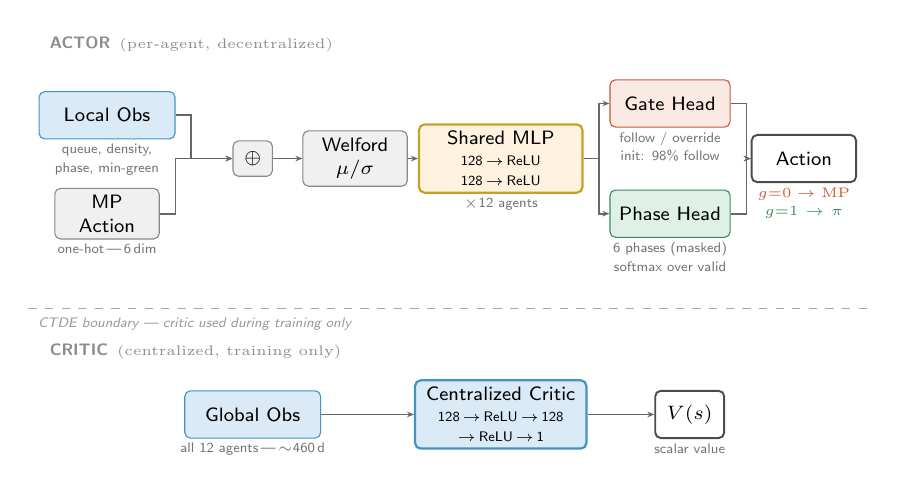
\begin{tikzpicture}[
    x=1cm, y=1cm,
    >={Stealth[length=2.5pt, width=2pt]},
    every node/.style={font=\sffamily},
    % --- node styles ---
    box/.style={
        draw, rounded corners=2pt, minimum height=0.6cm,
        inner sep=2.5pt, align=center,
        font=\sffamily\fontsize{7}{8.4}\selectfont,
    },
    inputbox/.style={box, fill=ascBlueFill, draw=ascBlue, text width=1.55cm},
    greybox/.style={box, fill=ascGreyFill, draw=ascGrey, minimum width=0.7cm},
    mlpbox/.style={box, fill=ascYellowFill, draw=ascYellow, line width=0.8pt,
                   text width=1.9cm, minimum height=0.8cm},
    gatebox/.style={box, fill=ascRedFill, draw=ascRed, text width=1.35cm},
    phasebox/.style={box, fill=ascGreenFill, draw=ascGreen, text width=1.35cm},
    actionbox/.style={box, draw=black!70, line width=0.7pt, text width=1.15cm},
    criticbox/.style={box, fill=ascBlueFill, draw=ascBlue, line width=0.8pt,
                      text width=2.0cm, minimum height=0.8cm},
    % --- annotation styles ---
    sub/.style={font=\sffamily\fontsize{5.5}{6.6}\selectfont,
                text=black!55, align=center, inner sep=0pt},
    arr/.style={->, semithick, color=black!60},
    trk/.style={font=\sffamily\bfseries\fontsize{6.5}{7.8}\selectfont,
                text=black!45},
]

% ===== ACTOR TRACK ==========================================================

\node[trk, anchor=west] at (0.15, 0.9)
    {ACTOR\enspace{\normalfont\fontsize{5.5}{6.6}\selectfont(per-agent, decentralized)}};

% -- Local Obs --
\node[inputbox] (lobs) at (1.0, 0) {Local Obs};
\node[sub, below=1.5pt of lobs.south, anchor=north, text width=2.0cm]
    {queue, density,\\phase, min-green};

% -- MP Action --
\node[greybox, text width=1.15cm] (mpact) at (1.0, -1.25) {MP Action};
\node[sub, below=1.5pt of mpact.south, anchor=north, text width=1.5cm]
    {one-hot\,|\,6\,dim};

% -- Concat --
\node[greybox, minimum width=0.5cm, minimum height=0.45cm,
      font=\sffamily\fontsize{7}{8.4}\selectfont] (cat) at (2.85, -0.55)
    {$\oplus$};

% -- Welford --
\node[greybox, text width=1.15cm] (welf) at (4.15, -0.55)
    {Welford $\mu/\sigma$};

% -- Shared MLP --
\node[mlpbox] (mlp) at (6.0, -0.55)
    {Shared MLP\\[-1pt]
     {\fontsize{5.5}{6.6}\selectfont 128\,$\to$\,ReLU}\\[-1pt]
     {\fontsize{5.5}{6.6}\selectfont 128\,$\to$\,ReLU}};
\node[sub, below=1.5pt of mlp.south, anchor=north]
    {$\times$12 agents};

% -- Gate Head --
\node[gatebox] (gate) at (8.15, 0.15) {Gate Head};
\node[sub, below=1.5pt of gate.south, anchor=north, text width=1.8cm]
    {follow / override\\init: 98\% follow};

% -- Phase Head --
\node[phasebox] (phase) at (8.15, -1.25) {Phase Head};
\node[sub, below=1.5pt of phase.south, anchor=north, text width=1.8cm]
    {6 phases (masked)\\softmax over valid};

% -- Action --
\node[actionbox] (act) at (9.85, -0.55) {Action};
\node[sub, below=1.5pt of act.south, anchor=north, text width=1.6cm]
    {{\color{ascRed}$g{=}0\!\to\!\mathrm{MP}$}\\
     {\color{ascGreen}$g{=}1\!\to\!\pi$}};

% -- Arrows: actor track --
\draw[arr] (lobs.east)  -- ++(0.2,0) |- (cat.west);
\draw[arr] (mpact.east) -- ++(0.2,0) |- (cat.west);
\draw[arr] (cat.east)   -- (welf.west);
\draw[arr] (welf.east)  -- (mlp.west);
\draw[arr] (mlp.east)   -- ++(0.2,0) |- (gate.west);
\draw[arr] (mlp.east)   -- ++(0.2,0) |- (phase.west);
\draw[arr] (gate.east)  -- ++(0.2,0) |- (act.west);
\draw[arr] (phase.east) -- ++(0.2,0) |- (act.west);


% ===== CTDE BOUNDARY ========================================================
\draw[dashed, black!35, line width=0.45pt] (0.0, -2.45) -- (10.7, -2.45);
\node[font=\sffamily\itshape\fontsize{5.5}{6.6}\selectfont, text=black!40,
      anchor=west] at (0.0, -2.65)
    {CTDE boundary --- critic used during training only};


% ===== CRITIC TRACK ==========================================================

\node[trk, anchor=west] at (0.15, -3.0)
    {CRITIC\enspace{\normalfont\fontsize{5.5}{6.6}\selectfont(centralized, training only)}};

% -- Global Obs --
\node[inputbox] (gobs) at (2.85, -3.8) {Global Obs};
\node[sub, below=1.5pt of gobs.south, anchor=north, text width=2.2cm]
    {all 12 agents\,|\,${\sim}$460\,d};

% -- Centralized Critic --
\node[criticbox] (crit) at (6.0, -3.8)
    {Centralized Critic\\[-1pt]
     {\fontsize{5.5}{6.6}\selectfont 128\,$\to$\,ReLU\,$\to$\,128}\\[-1pt]
     {\fontsize{5.5}{6.6}\selectfont $\to$\,ReLU\,$\to$\,1}};

% -- V(s) --
\node[actionbox, text width=0.7cm, minimum width=0.7cm] (vs) at (8.4, -3.8)
    {$V(s)$};
\node[sub, below=1.5pt of vs.south, anchor=north, text width=1.1cm]
    {scalar value};

% -- Arrows: critic track --
\draw[arr] (gobs.east) -- (crit.west);
\draw[arr] (crit.east) -- (vs.west);

\end{tikzpicture}
 inside a figure environment
% Requires: \usepackage{tikz} in the preamble
% Designed for NeurIPS two-column layout (\columnwidth ~ 3.25in)
\usetikzlibrary{arrows.meta, positioning, calc, backgrounds, fit}

% ---------------------------------------------------------------------------
% Colour palette
% ---------------------------------------------------------------------------
\definecolor{ascBlue}{HTML}{4393C3}
\definecolor{ascBlueFill}{HTML}{DAEAF6}
\definecolor{ascRed}{HTML}{C75B39}
\definecolor{ascRedFill}{HTML}{FBEAE4}
\definecolor{ascGreen}{HTML}{388E5E}
\definecolor{ascGreenFill}{HTML}{DFF0E7}
\definecolor{ascYellow}{HTML}{C8A028}
\definecolor{ascYellowFill}{HTML}{FFF3E0}
\definecolor{ascGrey}{HTML}{888888}
\definecolor{ascGreyFill}{HTML}{F0F0F0}

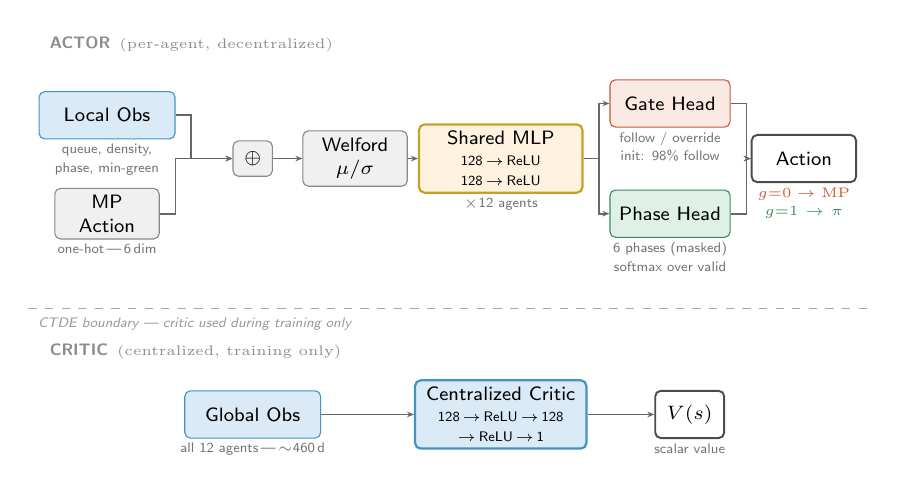
\begin{tikzpicture}[
    x=1cm, y=1cm,
    >={Stealth[length=2.5pt, width=2pt]},
    every node/.style={font=\sffamily},
    % --- node styles ---
    box/.style={
        draw, rounded corners=2pt, minimum height=0.6cm,
        inner sep=2.5pt, align=center,
        font=\sffamily\fontsize{7}{8.4}\selectfont,
    },
    inputbox/.style={box, fill=ascBlueFill, draw=ascBlue, text width=1.55cm},
    greybox/.style={box, fill=ascGreyFill, draw=ascGrey, minimum width=0.7cm},
    mlpbox/.style={box, fill=ascYellowFill, draw=ascYellow, line width=0.8pt,
                   text width=1.9cm, minimum height=0.8cm},
    gatebox/.style={box, fill=ascRedFill, draw=ascRed, text width=1.35cm},
    phasebox/.style={box, fill=ascGreenFill, draw=ascGreen, text width=1.35cm},
    actionbox/.style={box, draw=black!70, line width=0.7pt, text width=1.15cm},
    criticbox/.style={box, fill=ascBlueFill, draw=ascBlue, line width=0.8pt,
                      text width=2.0cm, minimum height=0.8cm},
    % --- annotation styles ---
    sub/.style={font=\sffamily\fontsize{5.5}{6.6}\selectfont,
                text=black!55, align=center, inner sep=0pt},
    arr/.style={->, semithick, color=black!60},
    trk/.style={font=\sffamily\bfseries\fontsize{6.5}{7.8}\selectfont,
                text=black!45},
]

% ===== ACTOR TRACK ==========================================================

\node[trk, anchor=west] at (0.15, 0.9)
    {ACTOR\enspace{\normalfont\fontsize{5.5}{6.6}\selectfont(per-agent, decentralized)}};

% -- Local Obs --
\node[inputbox] (lobs) at (1.0, 0) {Local Obs};
\node[sub, below=1.5pt of lobs.south, anchor=north, text width=2.0cm]
    {queue, density,\\phase, min-green};

% -- MP Action --
\node[greybox, text width=1.15cm] (mpact) at (1.0, -1.25) {MP Action};
\node[sub, below=1.5pt of mpact.south, anchor=north, text width=1.5cm]
    {one-hot\,|\,6\,dim};

% -- Concat --
\node[greybox, minimum width=0.5cm, minimum height=0.45cm,
      font=\sffamily\fontsize{7}{8.4}\selectfont] (cat) at (2.85, -0.55)
    {$\oplus$};

% -- Welford --
\node[greybox, text width=1.15cm] (welf) at (4.15, -0.55)
    {Welford $\mu/\sigma$};

% -- Shared MLP --
\node[mlpbox] (mlp) at (6.0, -0.55)
    {Shared MLP\\[-1pt]
     {\fontsize{5.5}{6.6}\selectfont 128\,$\to$\,ReLU}\\[-1pt]
     {\fontsize{5.5}{6.6}\selectfont 128\,$\to$\,ReLU}};
\node[sub, below=1.5pt of mlp.south, anchor=north]
    {$\times$12 agents};

% -- Gate Head --
\node[gatebox] (gate) at (8.15, 0.15) {Gate Head};
\node[sub, below=1.5pt of gate.south, anchor=north, text width=1.8cm]
    {follow / override\\init: 98\% follow};

% -- Phase Head --
\node[phasebox] (phase) at (8.15, -1.25) {Phase Head};
\node[sub, below=1.5pt of phase.south, anchor=north, text width=1.8cm]
    {6 phases (masked)\\softmax over valid};

% -- Action --
\node[actionbox] (act) at (9.85, -0.55) {Action};
\node[sub, below=1.5pt of act.south, anchor=north, text width=1.6cm]
    {{\color{ascRed}$g{=}0\!\to\!\mathrm{MP}$}\\
     {\color{ascGreen}$g{=}1\!\to\!\pi$}};

% -- Arrows: actor track --
\draw[arr] (lobs.east)  -- ++(0.2,0) |- (cat.west);
\draw[arr] (mpact.east) -- ++(0.2,0) |- (cat.west);
\draw[arr] (cat.east)   -- (welf.west);
\draw[arr] (welf.east)  -- (mlp.west);
\draw[arr] (mlp.east)   -- ++(0.2,0) |- (gate.west);
\draw[arr] (mlp.east)   -- ++(0.2,0) |- (phase.west);
\draw[arr] (gate.east)  -- ++(0.2,0) |- (act.west);
\draw[arr] (phase.east) -- ++(0.2,0) |- (act.west);


% ===== CTDE BOUNDARY ========================================================
\draw[dashed, black!35, line width=0.45pt] (0.0, -2.45) -- (10.7, -2.45);
\node[font=\sffamily\itshape\fontsize{5.5}{6.6}\selectfont, text=black!40,
      anchor=west] at (0.0, -2.65)
    {CTDE boundary --- critic used during training only};


% ===== CRITIC TRACK ==========================================================

\node[trk, anchor=west] at (0.15, -3.0)
    {CRITIC\enspace{\normalfont\fontsize{5.5}{6.6}\selectfont(centralized, training only)}};

% -- Global Obs --
\node[inputbox] (gobs) at (2.85, -3.8) {Global Obs};
\node[sub, below=1.5pt of gobs.south, anchor=north, text width=2.2cm]
    {all 12 agents\,|\,${\sim}$460\,d};

% -- Centralized Critic --
\node[criticbox] (crit) at (6.0, -3.8)
    {Centralized Critic\\[-1pt]
     {\fontsize{5.5}{6.6}\selectfont 128\,$\to$\,ReLU\,$\to$\,128}\\[-1pt]
     {\fontsize{5.5}{6.6}\selectfont $\to$\,ReLU\,$\to$\,1}};

% -- V(s) --
\node[actionbox, text width=0.7cm, minimum width=0.7cm] (vs) at (8.4, -3.8)
    {$V(s)$};
\node[sub, below=1.5pt of vs.south, anchor=north, text width=1.1cm]
    {scalar value};

% -- Arrows: critic track --
\draw[arr] (gobs.east) -- (crit.west);
\draw[arr] (crit.east) -- (vs.west);

\end{tikzpicture}
 inside a figure environment
% Requires: \usepackage{tikz} in the preamble
% Designed for NeurIPS two-column layout (\columnwidth ~ 3.25in)
\usetikzlibrary{arrows.meta, positioning, calc, backgrounds, fit}

% ---------------------------------------------------------------------------
% Colour palette
% ---------------------------------------------------------------------------
\definecolor{ascBlue}{HTML}{4393C3}
\definecolor{ascBlueFill}{HTML}{DAEAF6}
\definecolor{ascRed}{HTML}{C75B39}
\definecolor{ascRedFill}{HTML}{FBEAE4}
\definecolor{ascGreen}{HTML}{388E5E}
\definecolor{ascGreenFill}{HTML}{DFF0E7}
\definecolor{ascYellow}{HTML}{C8A028}
\definecolor{ascYellowFill}{HTML}{FFF3E0}
\definecolor{ascGrey}{HTML}{888888}
\definecolor{ascGreyFill}{HTML}{F0F0F0}

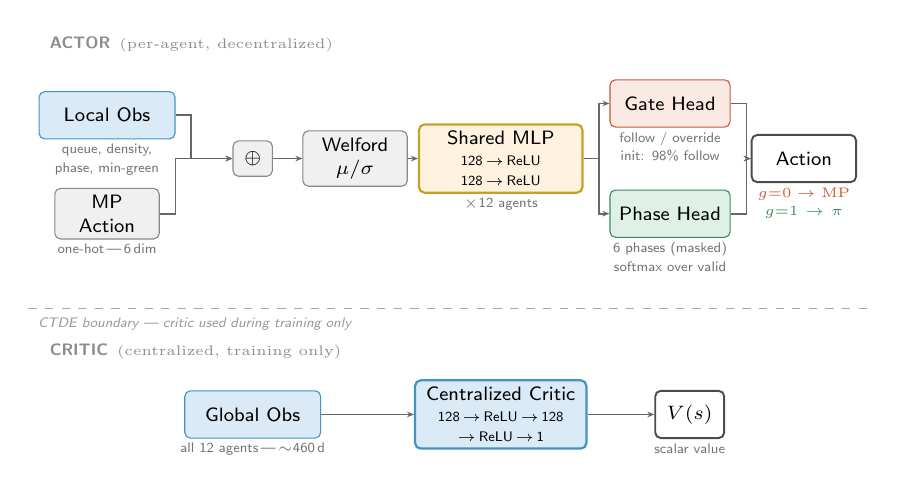
\begin{tikzpicture}[
    x=1cm, y=1cm,
    >={Stealth[length=2.5pt, width=2pt]},
    every node/.style={font=\sffamily},
    % --- node styles ---
    box/.style={
        draw, rounded corners=2pt, minimum height=0.6cm,
        inner sep=2.5pt, align=center,
        font=\sffamily\fontsize{7}{8.4}\selectfont,
    },
    inputbox/.style={box, fill=ascBlueFill, draw=ascBlue, text width=1.55cm},
    greybox/.style={box, fill=ascGreyFill, draw=ascGrey, minimum width=0.7cm},
    mlpbox/.style={box, fill=ascYellowFill, draw=ascYellow, line width=0.8pt,
                   text width=1.9cm, minimum height=0.8cm},
    gatebox/.style={box, fill=ascRedFill, draw=ascRed, text width=1.35cm},
    phasebox/.style={box, fill=ascGreenFill, draw=ascGreen, text width=1.35cm},
    actionbox/.style={box, draw=black!70, line width=0.7pt, text width=1.15cm},
    criticbox/.style={box, fill=ascBlueFill, draw=ascBlue, line width=0.8pt,
                      text width=2.0cm, minimum height=0.8cm},
    % --- annotation styles ---
    sub/.style={font=\sffamily\fontsize{5.5}{6.6}\selectfont,
                text=black!55, align=center, inner sep=0pt},
    arr/.style={->, semithick, color=black!60},
    trk/.style={font=\sffamily\bfseries\fontsize{6.5}{7.8}\selectfont,
                text=black!45},
]

% ===== ACTOR TRACK ==========================================================

\node[trk, anchor=west] at (0.15, 0.9)
    {ACTOR\enspace{\normalfont\fontsize{5.5}{6.6}\selectfont(per-agent, decentralized)}};

% -- Local Obs --
\node[inputbox] (lobs) at (1.0, 0) {Local Obs};
\node[sub, below=1.5pt of lobs.south, anchor=north, text width=2.0cm]
    {queue, density,\\phase, min-green};

% -- MP Action --
\node[greybox, text width=1.15cm] (mpact) at (1.0, -1.25) {MP Action};
\node[sub, below=1.5pt of mpact.south, anchor=north, text width=1.5cm]
    {one-hot\,|\,6\,dim};

% -- Concat --
\node[greybox, minimum width=0.5cm, minimum height=0.45cm,
      font=\sffamily\fontsize{7}{8.4}\selectfont] (cat) at (2.85, -0.55)
    {$\oplus$};

% -- Welford --
\node[greybox, text width=1.15cm] (welf) at (4.15, -0.55)
    {Welford $\mu/\sigma$};

% -- Shared MLP --
\node[mlpbox] (mlp) at (6.0, -0.55)
    {Shared MLP\\[-1pt]
     {\fontsize{5.5}{6.6}\selectfont 128\,$\to$\,ReLU}\\[-1pt]
     {\fontsize{5.5}{6.6}\selectfont 128\,$\to$\,ReLU}};
\node[sub, below=1.5pt of mlp.south, anchor=north]
    {$\times$12 agents};

% -- Gate Head --
\node[gatebox] (gate) at (8.15, 0.15) {Gate Head};
\node[sub, below=1.5pt of gate.south, anchor=north, text width=1.8cm]
    {follow / override\\init: 98\% follow};

% -- Phase Head --
\node[phasebox] (phase) at (8.15, -1.25) {Phase Head};
\node[sub, below=1.5pt of phase.south, anchor=north, text width=1.8cm]
    {6 phases (masked)\\softmax over valid};

% -- Action --
\node[actionbox] (act) at (9.85, -0.55) {Action};
\node[sub, below=1.5pt of act.south, anchor=north, text width=1.6cm]
    {{\color{ascRed}$g{=}0\!\to\!\mathrm{MP}$}\\
     {\color{ascGreen}$g{=}1\!\to\!\pi$}};

% -- Arrows: actor track --
\draw[arr] (lobs.east)  -- ++(0.2,0) |- (cat.west);
\draw[arr] (mpact.east) -- ++(0.2,0) |- (cat.west);
\draw[arr] (cat.east)   -- (welf.west);
\draw[arr] (welf.east)  -- (mlp.west);
\draw[arr] (mlp.east)   -- ++(0.2,0) |- (gate.west);
\draw[arr] (mlp.east)   -- ++(0.2,0) |- (phase.west);
\draw[arr] (gate.east)  -- ++(0.2,0) |- (act.west);
\draw[arr] (phase.east) -- ++(0.2,0) |- (act.west);


% ===== CTDE BOUNDARY ========================================================
\draw[dashed, black!35, line width=0.45pt] (0.0, -2.45) -- (10.7, -2.45);
\node[font=\sffamily\itshape\fontsize{5.5}{6.6}\selectfont, text=black!40,
      anchor=west] at (0.0, -2.65)
    {CTDE boundary --- critic used during training only};


% ===== CRITIC TRACK ==========================================================

\node[trk, anchor=west] at (0.15, -3.0)
    {CRITIC\enspace{\normalfont\fontsize{5.5}{6.6}\selectfont(centralized, training only)}};

% -- Global Obs --
\node[inputbox] (gobs) at (2.85, -3.8) {Global Obs};
\node[sub, below=1.5pt of gobs.south, anchor=north, text width=2.2cm]
    {all 12 agents\,|\,${\sim}$460\,d};

% -- Centralized Critic --
\node[criticbox] (crit) at (6.0, -3.8)
    {Centralized Critic\\[-1pt]
     {\fontsize{5.5}{6.6}\selectfont 128\,$\to$\,ReLU\,$\to$\,128}\\[-1pt]
     {\fontsize{5.5}{6.6}\selectfont $\to$\,ReLU\,$\to$\,1}};

% -- V(s) --
\node[actionbox, text width=0.7cm, minimum width=0.7cm] (vs) at (8.4, -3.8)
    {$V(s)$};
\node[sub, below=1.5pt of vs.south, anchor=north, text width=1.1cm]
    {scalar value};

% -- Arrows: critic track --
\draw[arr] (gobs.east) -- (crit.west);
\draw[arr] (crit.east) -- (vs.west);

\end{tikzpicture}
